\section{Tasks Status} % Seções são adicionadas para organizar sua apresentação em blocos discretos, todas as seções e subseções são automaticamente exibidas no índice como uma visão geral da apresentação, mas NÃO são exibidas como slides separados.

%----------------------------------------------------------------------------------------


\begin{frame}
  \frametitle{Tasks Status}

  % Ajustes úteis em tabelas no Beamer
  \centering
  \renewcommand{\arraystretch}{1.15} % mais espaço vertical entre linhas

  \begin{table}

\begin{tabular}{|p{0.58\textwidth}|c|p{0.22\textwidth}|}
\hline
\textbf{Task} & \textbf{Status} & \textbf{Link} \\
\hline

\textbf{Criar toy model} & &
\multirow{4}{*}{\centering \href{https://high-energy-physics-research.github.io/Gaussian-Process-Research/studies.html?nb=Estudo\%2FFase+01+-+Prova+de+Conceito\%2FModel-to-data-Comparison.ipynb}
     {Notebook}} \\
\cline{1-2}

\hspace{1.2em}\small$\hookrightarrow$ Gerar dados sintéticos (correlacionados + ruído opcional) & \done & \\
\cline{1-2}

\hspace{1.2em}\small$\hookrightarrow$ Ajustar GP (kernel, hiperparâmetros) & \done & \\
\cline{1-2}

\hspace{1.2em}\small$\hookrightarrow$ Comparar: resíduos, log-likelihood & \done & \\
\cline{1-2}

\hspace{1.2em}\small$\hookrightarrow$ Plotar a previsão & \done & \\
\hline
\end{tabular}
\end{table}
\end{frame}
%----------------------------------------------------------------------------------------


\begin{frame}
  \frametitle{Tasks Status}

  \centering
  \renewcommand{\arraystretch}{1.15}

  \begin{table}
    \begin{tabular}{|p{0.58\textwidth}|c|p{0.22\textwidth}|}
      \hline
      \textbf{Task} & \textbf{Status} &  \\
      \hline

      \textbf{Analisar toy model} &  &  \\
      \hline

      \hspace{1.2em}\small$\hookrightarrow$ Construção do modelo GP
      & \done &  \\
      \hline

      \hspace{1.2em}\small$\hookrightarrow$ Predição
      & \done &  \\
      \hline

      \hspace{1.2em}\small$\hookrightarrow$ Resíduos
      & \done &  \\
      \hline

      \hspace{1.2em}\small$\hookrightarrow$ Comparação entre incertezas experimentais e preditas
      & \done &  \\
      \hline

      \hspace{1.2em}\small$\hookrightarrow$ Estudo das incertezas correlacionadas e não correlacionadas, experimentais e preditas
      & \inprogress &  \\
      \hline

      \hspace{1.2em}\small$\hookrightarrow$ Aprendizado do kernel
      & \pending &  \\
      \hline

    \end{tabular}
  \end{table}
\end{frame}

\begin{frame}
  \frametitle{Tasks Status}

  % Ajustes úteis em tabelas no Beamer
  \centering
  \renewcommand{\arraystretch}{1.15} % mais espaço vertical entre linhas

  \begin{table}

\begin{tabular}{|p{0.58\textwidth}|c|p{0.22\textwidth}|}
\hline
\textbf{Task} & \textbf{Status} & \textbf{Link} \\
\hline

\textbf{Escrever projeto} & &
\multirow{4}{*}{\centering \href{https://www.overleaf.com/project/696e133a1101ac682ea3dd98}{Projeto}} \\
\cline{1-2}

\hspace{1.2em}\small$\hookrightarrow$ Definir escopo e objetivos & \done & \\
\cline{1-2}

\hspace{1.2em}\small$\hookrightarrow$ Esboçar introdução (motivação + observáveis) & \done & \\
\cline{1-2}

\hspace{1.2em}\small$\hookrightarrow$ Listar método/dados (GP, Inferencia Bayesiana) & \pending & \\
\cline{1-2}

\hspace{1.2em}\small$\hookrightarrow$ Listar objetivos & \inprogress & \\
\cline{1-2}

\hspace{1.2em}\small$\hookrightarrow$ Cronograma & \done & \\
\cline{1-2}

\hspace{1.2em}\small$\hookrightarrow$ Selecionar bibliografia & \done & \\
\hline
\end{tabular}
\end{table}
\end{frame}

% \begin{frame}{Uma imagem}
%     \frametitle{Historical Records}
%     In addition, it is possible to retrieve the full search history by running the script directly via GitHub Actions.
%    \begin{figure}[h]
%        \centering
%        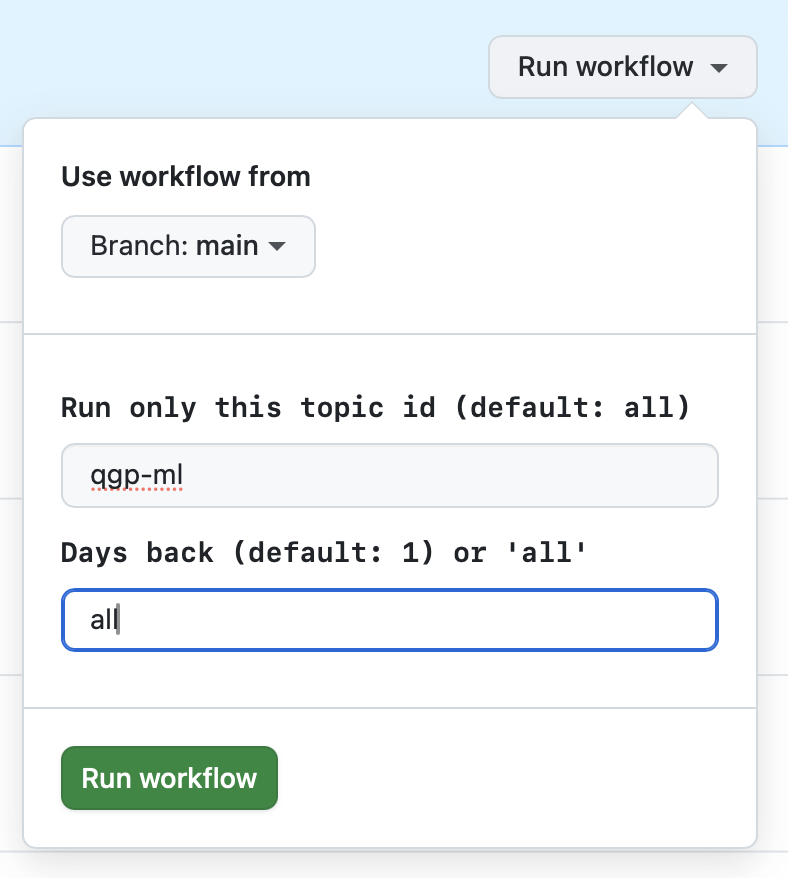
\includegraphics[width=0.3\textwidth]{img/github_topic_history.png}
%        \caption{GitHub Actions interface illustrating how the workflow can be executed to retrieve the full search history for a specific topic.}
%        \label{fig:github_topic_history}
%    \end{figure}
% \end{frame}
%----------------------------------------------------------------------------------------

% \begin{frame}
% 	\frametitle{Texto em tópicos}
%      Lorem ipsum dolor sit amet, consectetur adipiscing elit:
%     \begin{itemize}
%         \item Lorem ipsum dolor sit amet.
%         \item Lorem ipsum dolor sit amet.
%     \end{itemize}
	
% \end{frame}


